%%% displayed synchronous programs
\makeatletter
\def\BEP{\begin{trivlist}\item[]
  \if@minipage\else\vskip\parskip\fi
  \leftskip\@totalleftmargin \advance\leftskip by 1\parindent
  \rightskip\z@ \parindent\z@ \parfillskip\@flushglue \parskip\z@
  \@tempswafalse \def\par{\if@tempswa\hbox{}\fi\@tempswatrue\@@par}
  \obeylines \tt \small \catcode``=13 \@noligs\frenchspacing\@vobeyspaces}
\def\EEP{\end{trivlist}}
\makeatother

\def\pp#1{\texttt{\small{#1}}}
\newcommand{\PP}[1]{\noindent{\textit{\textbf{#1}}}}

\def\X#1{$x_{#1}$}
\def\B#1{\texttt{#1}}

\def\se{\textit{syn{\small ERJY}}}
\def\sec{\textit{syn{\small ERJYcharts}}}
\def\sef{\textit{syn{\scriptsize ERJY}}}
\def\argos{\textsc{Argos}}
\def\lustre{\textsc{Lustre}}
\def\signal{\textsc{Signal}}
\def\esterel{\textsc{Esterel}}
\def\statecharts{\textsc{Statecharts}}
\def\synccharts{\textsc{SyncCharts}}
\def\java{\textsc{Java}$^{\mbox{\tiny TM}}$}
\def\matlab{\textsc{MATLAB}$^{\mbox{\tiny TM}}$}

\newcommand{\GO}[0]{{\small GO}}
\newcommand{\GOs}[0]{{\small GO}s}
\newcommand{\spc}[0]{\vspace{0.2cm}}

\newcommand{\vs}[0]{\vspace{1pt}}
\newcommand{\NTI}[1]{\textit{#1}}
\newcommand{\NTD}[1]{{\em #1}\label{#1}}
\newcommand{\NT}[1]{\index{#1@{\em #1}}\hyperref{#1}{#1}{}{#1}}
\newcommand{\NTZ}[2]{\index{#1@{\em #1}}\hyperref{#1}{#1#2}{}{#1}}
\newcommand{\KWI}[1]{{\index{#1@{\tt #1}}\tt #1}}
\newcommand{\T}[1]{{\tt #1}}
\newcommand{\is}[0]{$\Rightarrow$\vs}
\newcommand{\mto}[0]{$\mapsto$}
\newcommand{\Bopt}[0]{{\bf (}}
\newcommand{\optE}[0]{{\bf )\opt}}
\newcommand{\opt}[0]{$_{\textit{\scriptsize opt~}}$}
\newcommand{\Balt}[0]{{\bf (}}
\newcommand{\alt}[0]{\,$|$}
\newcommand{\altE}[0]{{\bf )$_\mbox{\em alt~}$}}
\renewcommand{\altE}[0]{{\bf )~}}
\newcommand{\lst}[0]{{...~~}}
\newcommand{\lsep}[1]{...\fbox{\scriptsize #1}...~~}
\newcommand{\rr}[0]{\vs\makebox[7mm]{}}

\newtheorem{example}{\bf Example}[section]
\newenvironment{BNF}{}{}

\def\codeinput#1{\IfFileExists{../tex_input/se.#1}{\input ../tex_input/se.#1}{\begin{center}chpt\_\thechapter\_#1.se\end{center}} {\footnotesize(cf. \texttt{chpt\_\thechapter\_#1.se})}}

\def\codefragment#1{\IfFileExists{../tex_input/se.#1}{\input ../tex_input/se.#1}{\begin{center}chpt\_\thechapter\_#1.se\end{center}}}

\def\codeinputref#1{\IfFileExists{../tex_input/se.#1}{\input ../tex_input/se.#1}{\begin{center}ref\_#1.se\end{center}} {\footnotesize(cf. \texttt{ref\_#1.se})}}

\def\codeinputuser#1{\IfFileExists{../tex_input/se.#1}{\input ../tex_input/se.#1}{\begin{center}user\_#1.se\end{center}} {\footnotesize(cf. \texttt{user\_#1.se})}}

\def\A{\mbox{${\cal A}$}}
\def\C{\mbox{${\cal C}$}}
\def\D{\mbox{${\cal D}$}}
\def\E{\mbox{${\cal E}$}}
\def\F{\mbox{${\cal F}$}}
\def\H{\mbox{${\cal H}$}}
\def\I{\mbox{${\cal I}$}}
\def\L{\mbox{${\cal L}$}}
\def\M{\mbox{${\cal M}$}}
\def\P{\mbox{${\cal P}$}}
\def\Q{\mbox{${\cal Q}$}}
\def\R{\mbox{${\cal R}$}}
\def\S{\mbox{${\cal S}$}}
\def\V{\mbox{${\cal V}$}}

\def\ARROW#1#2{\mbox{\def\arraystretch{0.1}\begin{tabular}{c}
$\ \scriptstyle #1\ $\\
\rightarrowfill\\
$\ \scriptstyle #2\ $\end{tabular}}}

\def\mkTitle#1{
\title{
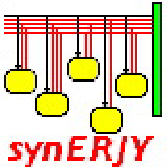
\includegraphics[height=50pt]{../pdf/se-logo}\hspace{0.5cm}
{\Huge \textit{\textbf{synERJY} 5.3}} \\ \vspace{1cm}\
       \textbf{#1}}

\author{\textit{Reinhard Budde}\\
\textit{Axel Poign\'e}\\
\textit{Karl-Heinz Sylla}\\
\ \\
\textbf{Fraunhofer Institut}\\\ \\ 
\textbf{Autonome intelligente Systeme}\\\ \\
\textbf{Fraunhofer AiS}\\\ \\\ \\
\\\ \\\ 
\\\  \\\ \\\ \\\ \\\ \\\textbf{\Large }
}

\date{\today}
}
